\documentclass[a4paper]{eccomas_paper-2024}

\usepackage{graphicx}
\usepackage{url}
\usepackage{amsmath}
\usepackage{amsfonts}
\usepackage{amssymb}
\usepackage{bm}
\usepackage{physics}

\usepackage{standalone}
\usepackage{booktabs}
\usepackage{pgfplotstable}
\pgfplotsset{compat=1.18}

\usepackage[%
backend=biber,
style=numeric, %alphabetic, numeric
giveninits=true,
natbib=true,
url=false,
doi=true,
eprint=false,
isbn=false,
defernumbers=true,
labelnumber,
hyperref=false,
maxbibnames=3,
sorting=none,%remove this to have things sorted, e.g. use style=alphabetic
]{biblatex}
\addbibresource{main.bib}
\addbibresource{references.bib}

\usepackage[commentmarkup=uwave]{changes}
\usepackage{xspace}

\definechangesauthor[color=blue, name={Philipp Diercks}]{pd}
\definechangesauthor[color=red, name={Joerg F. Unger}]{jfu}
\definechangesauthor[color=orange, name={Annika Robens-Radermacher}]{arr}

% custom commands
\newcommand{\ie}{i.\,e.\@\xspace}
\newcommand{\eg}{e.\,g.\@\xspace}

\title{AN EFFICIENT LOCALIZED MODEL ORDER REDUCTION FRAMEWORK FOR THE SHAPE OPTIMIZATION OF ADDITIVELY MANUFACTURED LATTICE STRUCTURES\break ECCOMAS CONGRESS 2024}

\author{Philipp Diercks$^{1}$, Karen Veroy$^{2}$, Annika Robens-Radermacher$^{1}$ and Jörg F. Unger$^{1}$}

% heading is supposed to contain only the authors (on all pages except the first page)
\heading{Philipp Diercks, Karen Veroy, Annika Robens-Radermacher and Jörg F. Unger}

\address{$^{1}$ Bundesanstalt für Materialforschung und -prüfung, Unter den Eichen 87, 12205 Berlin, \{philipp.diercks, annika.robens-radermacher, joerg.unger\}@bam.de, \url{www.bam.de}
\and
$^{2}$ Centre for Analysis, Scientific Computing and Applications (CASA), Department of Mathematics and Computer Science, TU Eindhoven, P.O. Box 513, 5600 MB Eindhoven, The Netherlands, k.p.veroy@tue.nl}

\keywords{Multiscale methods, Domain decomposition methods, Model order reduction, parameterized PDEs, Shape optimization}

% TODO abstract
\abstract{\comment[id=pd]{TODO: add abstract}.}

\begin{document}
\thispagestyle{empty}

\section{INTRODUCTION}%
\label{sec:introduction}

Additive manufacturing (AM), commonly known as 3D printing, is a manufacturing technique that allows for the production of a wide range of structures and complex geometries.
The objects are build successively by adding material layer by layer from three-dimensional models.
The technology offers numerous advantages over conventional manufacturing, including greater design flexibility, reduced material waste, and the possibility to produce complex structures with tailored material properties.
It has been used in a wide range of applications, including aerospace, biomechanical, automotive, and construction industries~\cite{Plessis2022Properties,Wu2016critical}.

A common engineering practice is to optimize the geometry of a structure by an iterative process, in which an objective function is minimized by systematically choosing parameter values $\bm\mu$ (design variables) and computing the value of the function.
In structural mechanics, a prominent example of an objective function is mass or compliance which is a function of the parameter-dependent displacement field $\bm{u}(\bm\mu)$.
In each iteration of the optimization process, the geometry is manually changed in the CAD model and the high fidelity finite element (FE) model, also called full order model (FOM), is simply re-evaluated.
While this approach is not only an ineffective use of resources, it is also infeasible when solving the FE model is a computationally demanding task, \eg{} in multiscale or large-scale industrial applications.
Due to the prohibitive cost of even a single FOM solution, the iterative design process cannot be performed using direct numerical simulations.
Therefore, we propose a framework based on localized, also called component-based (CB), parametric model order reduction (pMOR).
The main idea is to precompute, in a localized manner, empirical basis functions which approximate the solution for some part of the domain without the need to solve the global FOM even once.
The global approximation is obtained by a suitable coupling of the local reduced spaces spanned by the aforementioned basis functions, in which one naturally relies on domain decomposition (DD) strategies.
For a review of concepts in localized model order reduction it is referred to~\cite{BuhrReview}.
In particular, regarding lattice structures, this approach allows to take advantage of the repetitiveness of the lattice, such that a computation of the local basis is required only for few components, \ie{} unit cells.

The computation of the local basis is an essential task in localized pMOR and is often done using the concept of oversampling~\cite{Hou1997Multiscale}.
In this approach, the target subdomain $\varOmega_{\mathrm{in}}$, \ie{} that part of the domain for which one would like to construct basis functions, is extended and boundary conditions are prescribed on the boundary of the larger so-called oversampling domain $\varOmega$ to explore possible solutions.
In the literature, this oversampling problem is also expressed in terms of a \textit{transfer operator} $\bm{T}$ that maps the values on the boundary $\partial\varOmega$ to the unknown solution restricted to the target subdomain $\bm{u}(\bm{\mu})\vert_{\varOmega_{\mathrm{in}}}$.
The construction of (optimal) local approximation spaces then comprises the calculation of the left singular vectors of this transfer operator~\cite{Babuska2011Optimal,Smetana2016Optimal}.
The direct calculation via eigenvalue problems is, however, computationally expensive and the range of the transfer operator, and thus the optimal local approximation spaces can be efficiently approximated by random sampling~\cite{Buhr2018Randomized}.
Here, the authors treat non-parametrized PDEs and to the authors knowledge the extension to the parametric setting for linear problems has not been done yet.
In~\cite{Smetana2016Optimal}, the authors propose a spectral greedy algorithm to construct local approximation spaces.
Taddei and Patera~\cite{Taddei2018Localization} propose a combination of transfer eigenproblems and proper orthogonal decomposition (POD).
For parameterized nonlinear elliptic PDEs Smetana and Taddei~\cite{Smetana2023Localized} present a randomized local training procedure with global enrichment.

The contributions of the present work are given as follows.
First, as references~\cite{Smetana2016Optimal,Taddei2018Localization} do not make use of range approximation via random sampling, suitable training strategies to construct local approximation spaces for parameterized linear problems via random sampling are investigated.
In particular, the approach given in~\cite{Taddei2018Localization}, identified as a \textit{distributed approximate POD} (see also~\cite{Himpe2018Hierarchical}), is compared to a \textit{heuristic randomized range finder} developed in this work.
Second, a framework for the shape optimization of lattice structures is proposed.
It combines the aforementioned algorithms to construct local approximation spaces with an auxiliary problem, as in~\cite{Guo2022Learning}, to facilitate geometrical parametrizations of the unit cell and the matrix version~\cite{Negri2015Efficient} of the empirical interpolation method (EIM)~\cite{Barrault2004‘empirical,Chaturantabut2010Nonlinear} to ensure online efficiency of the final reduced order model.
Furthermore, the global approximation space is constructed from the local spaces using the generalized finite element method (GFEM)~\cite{Babuska2004Generalized}.

% TODO add paragraph outlining structure of the text

\section{METHOD}%
\label{sec:method}

\subsection{Auxiliary Problem} % (fold)
\label{sub:Auxiliary Problem}

% subsection Auxiliary Problem (end)

\subsection{Construction of local approximation spaces} % (fold)
\label{sub:Construction of local approximation spaces}

% subsection Construction of local approximation spaces (end)

\subsubsection{Randomized range finder and proper orthogonal decomposition} % (fold)
\label{sec:Randomized range finder and POD}

% subsubsection Randomized range finder and POD (end)

\subsubsection{Heuristic randomized range finder} % (fold)
\label{sec:Heuristic randomized range finder}

% subsubsection Heuristic randomized range finder (end)

\subsection{Construction of a global approximation} % (fold)
\label{sub:Construction of a global approximation}

% subsection Construction of a global approximation (end)

\subsection{Online efficiency} % (fold)
\label{sub:Online efficiency}

% subsection Online efficiency (end)

\section{NUMERICAL EXPERIMENTS} % (fold)
\label{sec:numerical experiments}

% section numerical experiments (end)

\subsection{Graded concrete slab} % (fold)
\label{sub:Graded concrete slab}

% \begin{figure}
%     \begin{center}
%         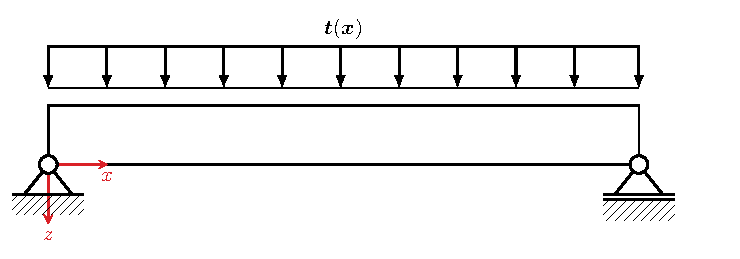
\includegraphics[width=0.95\textwidth]{./figures/beam/beam_sketch.pdf}
%     \end{center}
%     \caption{Schematic representation of the structural problem. A simply supported beam is subjected to a constant load.}\label{fig:beam_sketch}
% \end{figure}
%
% TODO placement
% \begin{figure}
%     \begin{center}
%         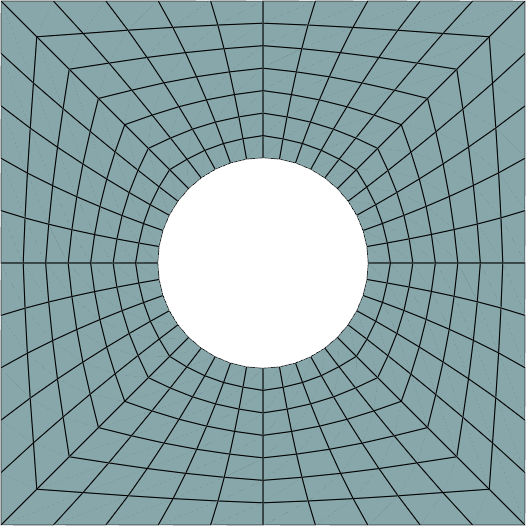
\includegraphics[width=0.65\textwidth]{./figures/beam/unit_cell.png}
%     \end{center}
%     \caption{Unit cell domain partition.}\label{fig:unit_cell_domain}
% \end{figure}
%
% \begin{figure}
%     \begin{center}
%         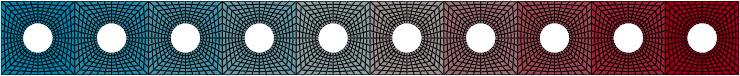
\includegraphics[width=0.95\textwidth]{./figures/beam/global_domain.png}
%     \end{center}
%     \caption{The partition of the global domain. The colors indicate the variation in Young's modulus for each subdomain.}\label{fig:global_domain}
% \end{figure}
%
% subsection Graded concrete slab (end)

\subsection{Projection error study} % (fold)
\label{sub:Projection error study}

% subsection Projection error study (end)

\subsection{Reduced order model validation} % (fold)
\label{sub:Reduced order model validation}

% subsection Reduced order model validation (end)

\subsection{Shape optimization} % (fold)
\label{sub:Shape optimization}

% subsection Shape optimization (end)

\section{CONCLUSIONS} % (fold)
\label{sec:conclusions}

% section CONCLUSION (end)

% \begin{figure}[!htb]
% \minipage{0.49\textwidth}
%   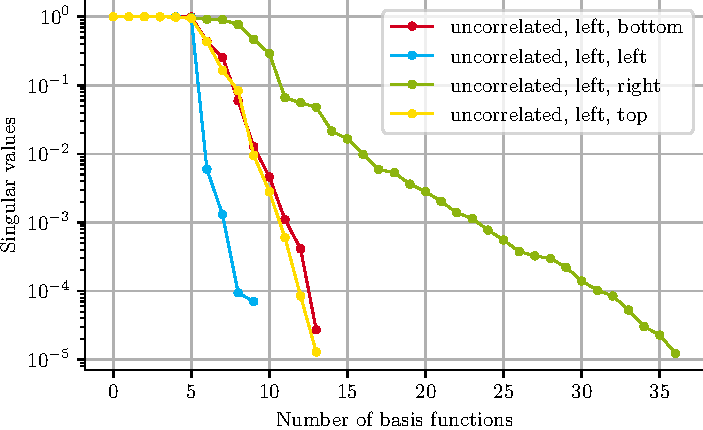
\includegraphics[]{./figures/beam/fig_loc_svals_left.pdf}
%   \caption{Singular valus left}\label{fig:loc_svals_left}
% \endminipage\hfill
% \minipage{0.49\textwidth}
%   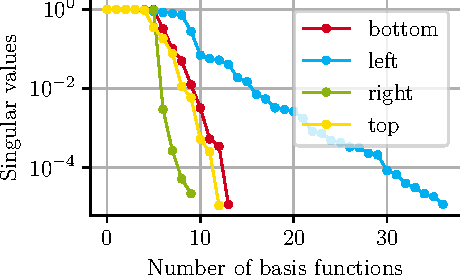
\includegraphics[]{./figures/beam/fig_loc_svals_right.pdf}
%   \caption{Singular valus right}\label{fig:loc_svals_right}
% \endminipage\hfill\\%
% \begin{center}
% \minipage{0.49\textwidth}
%   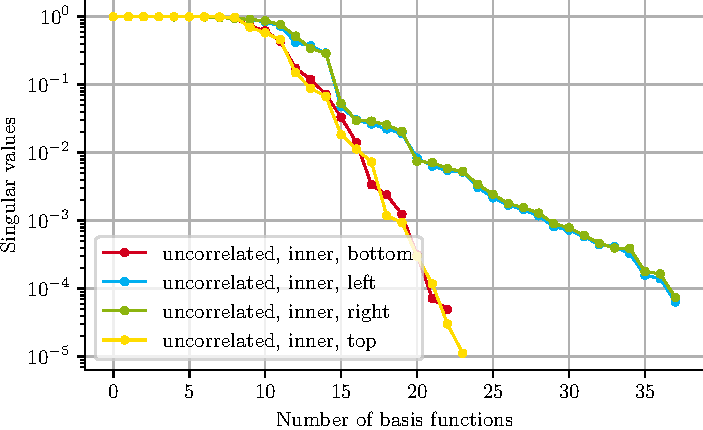
\includegraphics[]{./figures/beam/fig_loc_svals_inner.pdf}
%   \caption{Singular valus inner}\label{fig:loc_svals_inner}
% \endminipage
% \end{center}
% \end{figure}


% \begin{figure}[!htb]
% \minipage{0.49\textwidth}
%   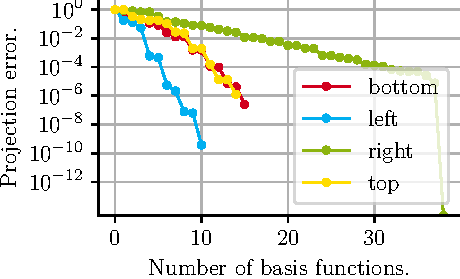
\includegraphics{./figures/beam/fig_proj_error_left_hapod.pdf}
%   \caption{Projection error hapod}\label{fig:proj_error_left_hapod}
% \endminipage\hfill
% \minipage{0.49\textwidth}
%   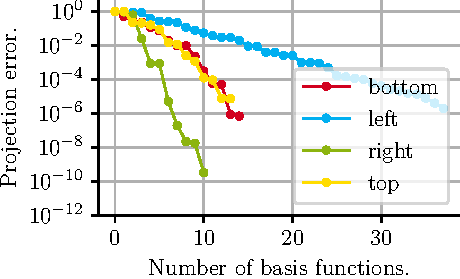
\includegraphics{./figures/beam/fig_proj_error_right_hapod.pdf}
%   \caption{Projection error hapod}\label{fig:proj_error_right_hapod}
% \endminipage\hfill\\
% \begin{center}
% \minipage{0.49\textwidth}%
%   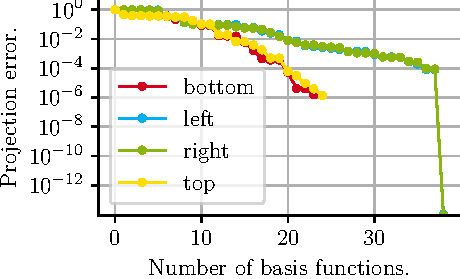
\includegraphics{./figures/beam/fig_proj_error_inner_hapod.pdf}
%   \caption{Projection error hapod}\label{fig:proj_error_inner_hapod}
% \endminipage
% \end{center}
% \end{figure}

% \begin{table}
%     \centering
%     \caption{HAPOD inner}\label{tab:hapod_inner}
%     \documentclass{standalone}

\usepackage{booktabs}
\usepackage{pgfplotstable}
\pgfplotsset{compat=1.18}

\begin{document}

\pgfplotstabletypeset[
  col sep=comma, % the seperator in our .csv file
  every head row/.style={
    before row={\toprule}, % have a rule at top
    after row={\midrule}
    },
  every last row/.style={after row=\bottomrule}, % rule at bottom
  column type=r,
  columns/Edge/.style={string type,column type=l},
]{../../../work/beam/hapod_table_inner.csv}

\end{document}

% \end{table}

% \begin{figure}[!htb]
% \minipage{0.49\textwidth}
%   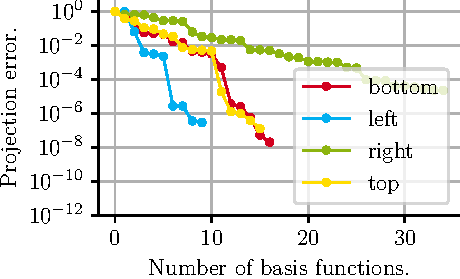
\includegraphics{./figures/beam/fig_proj_error_left_heuristic.pdf}
%   \caption{Projection error }\label{fig:proj_error_left_heuristic}
% \endminipage\hfill
% \minipage{0.49\textwidth}
%   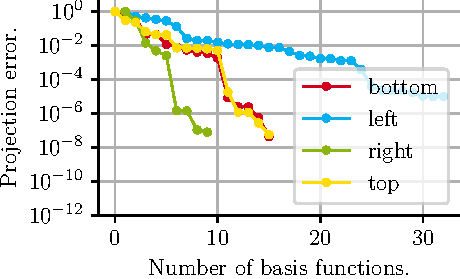
\includegraphics{./figures/beam/fig_proj_error_right_heuristic.pdf}
%   \caption{Projection error }\label{fig:proj_error_right_heuristic}
% \endminipage\hfill\\
% \begin{center}
% \minipage{0.49\textwidth}%
%   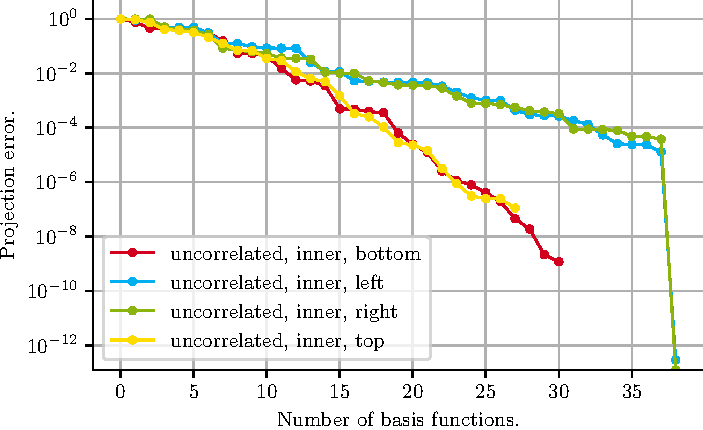
\includegraphics{./figures/beam/fig_proj_error_inner_heuristic.pdf}
%   \caption{Projection error }\label{fig:proj_error_inner_heuristic}
% \endminipage
% \end{center}
% \end{figure}

% \begin{table}
%     \centering
%     \caption{Heuristic rrf inner}\label{tab:heuristic_inner}
%     \documentclass{standalone}

\usepackage{booktabs}
\usepackage{pgfplotstable}
\pgfplotsset{compat=1.18}

\begin{document}

\pgfplotstabletypeset[
  col sep=comma, % the seperator in our .csv file
  every head row/.style={
    before row={\toprule}, % have a rule at top
    after row={\midrule}
    },
  every last row/.style={after row=\bottomrule}, % rule at bottom
  column type=r,
  columns/Edge/.style={string type,column type=l},
]{../../../work/beam/heuristic_table_inner.csv}

\end{document}

% \end{table}

% \begin{figure}[!htb]
%     \centering
%     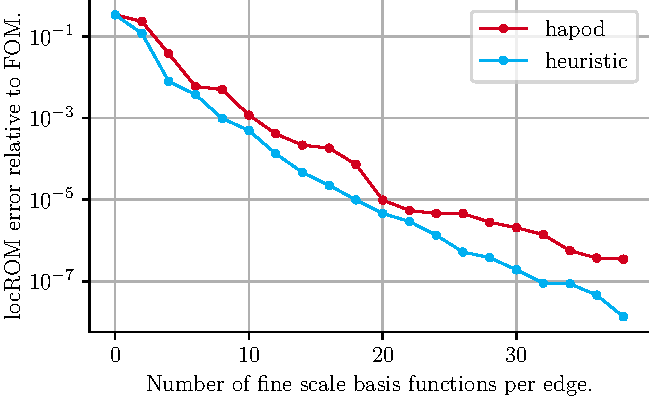
\includegraphics{./figures/beam/fig_loc_rom_error.pdf}
%     \caption{Local ROM error relative to FOM.}\label{fig:loc_rom_error}
% \end{figure}

% \begin{table}
%     \caption{Result of the optimization with FOM and ROM.}\label{tab:minimization_data}
%     \centering
%     \documentclass{standalone}

\usepackage{booktabs}
\usepackage{siunitx}
\usepackage{pgfplotstable}
\pgfplotsset{compat=1.18}

% Setup siunitx:
\sisetup{
  round-mode          = places, % Rounds numbers
  round-precision     = 2, % to 2 places
}

\begin{document}

\pgfplotstabletypeset[
  col sep=comma,
  % columns={Model,Iterations,Evaluations,Time,{Output J}},
  display columns/3/.style={column name={Time}, precision=3},
  display columns/4/.style={column name={Output $J$}, sci zerofill, precision=3},
  every head row/.style={
    before row={\toprule}, % have a rule at top
    % set unit for each column
    after row={
        & - & - & \si{\second} & \si{\newton\milli\metre}\\
    \midrule}
    },
  every last row/.style={after row=\bottomrule}, % rule at bottom
  column type=r,
  columns/Model/.style={string type,column type=l},
]{./work/beam/minimization_data.csv}

\end{document}

% \end{table}

% \begin{table}
%     \caption{Comparison of reduced optimal solution $\mu_N^{\ast}$ and true optimal solution $\mu^{\ast}$.}\label{tab:minimization_comparison}
%     \centering
%     \documentclass{standalone}

\usepackage{booktabs}
\usepackage{siunitx}
\usepackage{pgfplotstable}
\usepackage{amsmath,physics}
\pgfplotsset{compat=1.18}

% Setup siunitx:
\sisetup{
  round-mode          = places, % Rounds numbers
  round-precision     = 2, % to 2 places
}

\begin{document}

\pgfplotstabletypeset[
  % FIXME using column type {S} does not lead to desired result 
  % columns/{Beam example}/.style={
  %     column type={S},
  %     sci zerofill,
  %     precision=3,
  % },
  multicolumn names,
  col sep=comma,
  column type=r,
  % columns={Model,Iterations,Evaluations,Time,{Output J}},
  display columns/0/.style={string type, column name={}, column type=l},
  display columns/1/.style={string type, column name={}, column type=l},
  display columns/2/.style={column name={Beam example}, sci zerofill, precision=4},
  every head row/.style={
    before row={\toprule}, % have a rule at top
    after row={\midrule},
    },
  every last row/.style={after row=\bottomrule}, % rule at bottom
]{./work/beam/minimization_comparison.csv}

\end{document}

% \end{table}

% references
\printbibliography[title=REFERENCES]

\end{document}
